\section{Overview}
\label{overview}
\subsection{Long-lived particles at the LHC}
As discussed in Section~\ref{llps}, LLPs are common in the SM and naturally arise in many BSM scenarios. When produced in proton-proton collisions at the LHC, new LLPs have the potential to produce striking experimental signatures that differentiate them from SM backgrounds. As diagrammed in Fig.~\ref{llp_signatures}, new LLPs that decay within the detector volume can produce displaced vertices, physics objects whose trajectories do not point back to the location of the proton-proton collision, or particle tracks that vanish before reaching the outer edge of the tracker. Neutral LLPs that decay farther out can pass undetected through the tracker before producing signals in the calorimeters or muon system, and heavy, charged LLPs that are stable on detector length scales can be identified by their unusually large charge depositions.

\begin{figure}[hbtp]
\centering
\includegraphics[scale=0.4]{figures/overview/llp_signatures.pdf}
\caption{Illustration of several possible experimental signatures of long-lived particles. Image courtesy of Jamie Antonelli.} 
\label{llp_signatures}
\end{figure}

The identification of any of these LLP signatures above the expected background rates would be a clear sign of new physics, but their atypical nature adds an inherent layer of difficulty to studying such signatures. In fact, standard reconstruction algorithms and event selections frequently discard such unusual signatures and render the majority of LHC analyses insensitive to many BSM scenarios that include LLPs~\cite{llp_whitepaper}. As a solution to the naturalness problem may require new physics at the LHC energy scale, it is critical that physicists face the challenges posed by LLP analyses and look everywhere BSM physics may be hiding.

Interest in LLPs is growing as evidence of BSM physics continues to evade LHC physicists. Recent CMS searches in \SI{13}{\TeV} proton-proton collisions target disappearing tracks~\cite{disappearing_tracks} or use the ECAL timing capabilities to target photons or jets whose production at a displaced vertex delays the time of their detection~\cite{delayed_photons, delayed_jets}. All observations thus far agree with SM predictions, but these and other LLP analyses are probing regions of BSM parameter space that are untested by conventional analyses.

\subsection{Displaced leptons signature}
The Displaced Leptons analysis targets electrons and muons produced in the decays of new LLPs. Inspired by models such as Displaced SUSY (see Section~\ref{displaced_susy}), we take care to maintain sensitivity to leptons that are produced in separate long-lived decays as well as those that share a common displaced vertex. This goal is achieved by selecting pairs of leptons with large transverse impact parameters and setting no constraints on the presence or absence of displaced vertices. Figure~\ref{displaced_leptons_cartoon} shows the benefit of such an approach: the pair-produced new LLPs, labeled $X$, each decay to a single lepton and an unspecified second particle. The lepton transverse impact parameter, which is labeled $d_0$ in the figure and defined explicitly below, is then used to identify the displaced nature of the lepton decays without explicitly constraining the other decay products in any way. Note also that the same strategy would successfully identify two leptons from a single long-lived particle decay.

\begin{figure}
\centering
\includegraphics[width=0.7\textwidth]{figures/overview/signalEventDisplay.pdf}
\caption{Illustration of the displaced leptons signature showing the definition of $d_0$ in a transverse view of the CMS detector. $X$ denotes a new long-lived particle, $\ell$ denotes an electron or muon, and $Y$ denotes any other decay products of the new long-lived particle. When interpreting the results of the Displaced Leptons analysis with the Displaced SUSY model, $X$ refers to a top squark and $Y$ refers to a b or d quark.} 
\label{displaced_leptons_cartoon}
\end{figure}

Lepton transverse impact parameter, $d_0$, is defined as the distance of closest approach in the transverse plane of the helical trajectory of the lepton track to the CMS beamspot, which is the center of the region in which the proton bunches cross. $d_0$ is commonly measured with respect to the primary vertex, but in the case of leptons produced in displaced decays, the association between a given primary vertex and the resulting leptons is unreliable. We determine $d_0$ from measured properties of the lepton track using the following equation:
\begin{equation}
    d_0 = \frac{(v_x - x_0)p_y - (v_y - y_0)p_x}{\pt}
\end{equation}
where $v_x$ and $v_y$ refer to the $x$ and $y$ coordinates of the lepton track reference point, which is usually chosen to be the point of closest approach to the center of CMS, $x_0$ and $y_0$ refer to the $x$ and $y$ coordinates of the beamspot, and $p_x$, $p_y$, and \pt refer to the magnitudes of the $x$, $y$, and transverse components of the lepton's momentum. \ad is commonly used throughout the Displaced Leptons analysis because we generally care about the magnitude of $d_0$ but not its direction.

If we are to use lepton \ad as the discriminating variable in an LLP search, we must ensure it scales appropriately with the parent LLP lifetime. Typically, a particle with lifetime $\tau$ will travel a distance $d=\beta\gamma c \tau$, where $\beta$ and $\gamma$ are relativistic factors and $c$ is the speed of light, so $d$ and $\tau$ are directly correlated. Figure~\ref{displaced_leptons_cartoon} shows that lepton \ad is determined by the distance travelled by the new LLP in the transverse plane and the angle between the transverse momenta of the new LLP and the lepton. Unless this angle is pathologically constrained to zero, \ad and $\tau$ will be directly correlated as well. In fact, the maximum value of lepton \ad, which occurs when the angle between the transverse momenta of the new LLP and the lepton is $\frac{\pi}{2}$, is exactly equal to the transverse distance between the beamspot and location of the LLP decay.

Figure~\ref{d0_discriminating_power} shows the distribution of data and simulated Displaced SUSY events in the plane defined by electron and muon \ad. As expected, the data events, which are dominated by leptons from promptly decaying parent particles, are concentrated at low \ad values while the Displaced SUSY events are spread across the entire plane. This figure shows the power of \ad as a discriminating variable: requiring two leptons with $\ad>\SI{100}{\um}$ eliminates nearly all the SM background without requiring that the leptons form a common vertex.

\begin{figure}[hbtp]
\centering
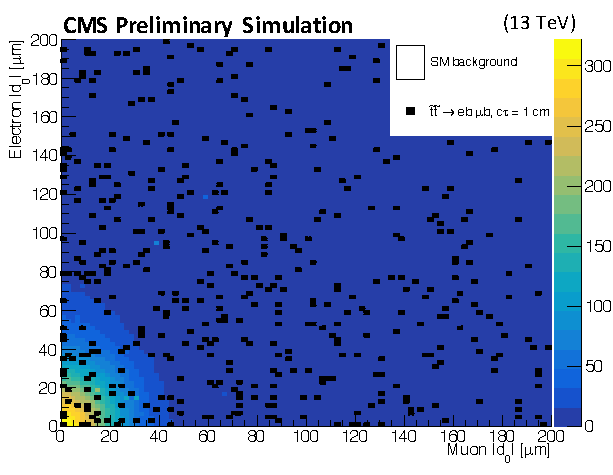
\includegraphics[scale=1.2]{figures/overview/d0_discriminating_power.pdf}
\caption{} 
\label{d0_discriminating_power}
\end{figure}
\fxnote{this is an ugly plot}

Another possible discriminating variable could be $\ad/\sigma_{\ad}$, where $\sigma_{\ad}$ is the uncertainty in \ad. Such a discriminating variable could potentially reduce the background from leptons with poorly measured \ad, but we choose to use \ad because of its straightforward correspondence to the parent particle lifetime. We also find that $\sigma_{\ad}$ is often underestimated, which reduces the potential benefit of using $\ad/\sigma_{\ad}$.

\subsection{Analysis strategy}
Having seen that \ad can be used to identify leptons from long-lived particle decays without requiring that the leptons form a common vertex, we now define a strategy to target such a signature. The basic analysis strategy is outlined here and described in detail in the following sections.

In addition to maximizing our sensitivity to models such as Displaced SUSY, we also strive to develop an analysis that is model independent, signature based, and easy to reinterpret. With these goals in mind, we perform a relatively simple cut-and-count analysis in which our main event selection sets no constraints on any non-lepton physics object. Unlike previous displaced leptons analyses~\cite{displaced_leptons_run1, displaced_leptons_bing}, we allow final states with more than two leptons and set no constraints on the lepton charge. As explained in Section~\ref{selection}, we select events in three analysis channels: electron-electron (\Pe\Pe), electron-muon (\Pe\Pgm), and muon-muon (\Pgm\Pgm). We then divide the events into different regions of the plane defined by the \ad of the two leptons that define the analysis channel. Figure~\ref{d0_discriminating_power}, for example, shows this plane in the $\Pe\Pgm$ channel. The signal region is defined as the region in which both leptons have $\ad>\SI{100}{\um}$.

Following the procedure defined in Section~\ref{bg}, we use the data in the non-signal regions to estimate the SM background in the signal region. Finally, we compare the background estimates and data yields in the signal region. In the absence of a significant excess, we use simulated signal events to constrain the available parameter space of the Displaced SUSY model. To avoid biasing the result, we blind ourselves to the data in the signal region and wait to observe the signal-region data until after we define and test the entire analysis procedure and receive pre-approval from the CMS Exotica Physics Analysis Group.

\pagebreak